%##noBuild

\section{Tabele}

\subsection{OSOBY}
\begin{verbatim}
CREATE TABLE OSOBY
(
 ID_OSOBY INT GENERATED ALWAYS AS IDENTITY NOT NULL
, IMIE VARCHAR2(50)
, NAZWISKO VARCHAR2(50)
, PESEL VARCHAR2(11)
, KONTAKT VARCHAR2(100)
, CONSTRAINT OSOBY_PK PRIMARY KEY
 (
 ID_OSOBY
 )
 ENABLE
);
\end{verbatim}

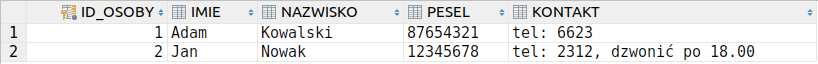
\includegraphics[width=\linewidth]{./images/osoby.png}

\subsection{WYCIECZKI}
\begin{verbatim}
CREATE OR REPLACE TABLE WYCIECZKI
(
 ID_WYCIECZKI INT GENERATED ALWAYS AS IDENTITY NOT NULL
, NAZWA VARCHAR2(100)
, KRAJ VARCHAR2(50)
, DATA DATE
, OPIS VARCHAR2(200)
, LICZBA_MIEJSC INT
, CONSTRAINT WYCIECZKI_PK PRIMARY KEY
 (
 ID_WYCIECZKI
 )
 ENABLE
);
\end{verbatim}


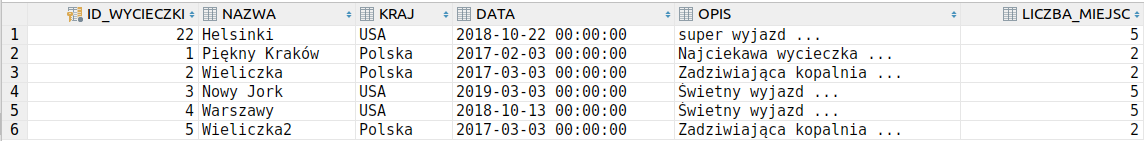
\includegraphics[width=\linewidth]{./images/wycieczki.png}

\subsection{REZERWACJE}
\begin{verbatim}
CREATE OR REPLACE TABLE REZERWACJE
(
 NR_REZERWACJI INT GENERATED ALWAYS AS IDENTITY NOT NULL
, ID_WYCIECZKI INT
, ID_OSOBY INT
, STATUS CHAR(1)
, CONSTRAINT REZERWACJE_PK PRIMARY KEY
 (
 NR_REZERWACJI
 )
 ENABLE
);
\end{verbatim}

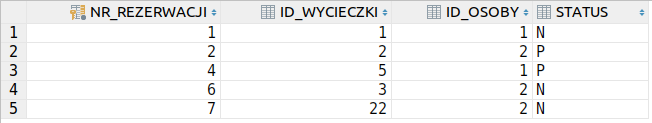
\includegraphics[width=\linewidth]{./images/przyszle_rezerwacje_osoby_rezerwacje.png}